\documentclass[a4paper, 12pt]{article}
\usepackage{./common/style}
\usepackage{graphicx}
\usepackage{placeins}
\usepackage[justification=centering]{caption}

\let\Oldsection
\section{\renewcommand{\section}{\FloatBarrier\Oldsection}}

\let\Oldsubsection
\subsection{\renewcommand{\subsection}{\FloatBarrier\Oldsubsection}}

\let\Oldsubsubsection
\subsubsection{\renewcommand{\subsubsection}{\FloatBarrier\Oldsubsubsection}}

\begin{document}
	\sloppy \docNumber{RU.17701729.05.06-01 34 01} \docFormat{Руководство оператора} \student{программы \enquote{Программная инженерия}}{Д.А. Щербаков} \project{Программа для визуализации данных о климате и погоде помощью JavaScript.}
	\supervisor{Доцент департамента программной инженерии}{Р.А. Родригес Залепинос} \firstPage
	\newpage
	\thirdPage

	\section{Назначение программы}
	\subsection{Функциональное назначение}
	Основное функциональное назначение программы заключается в загрузке, обработке и визуализации данных о климате и
	погоде. Программа должна реализовывать следующие основные функции:
	\begin{itemize}
		\item \textbf{Загрузка и обработка данных:} Программа должна уметь загружать и обрабатывать данные о климате и
			погоде из различных источников, включая открытые метеорологические базы данных и пользовательские файлы.

		\item \textbf{Визуализация данных:} Программа должна предоставлять средства для визуализации климатических и
			погодных данных с использованием графиков и географических карт.

		\item \textbf{Фильтрация и сортировка данных:} Пользователи должны иметь возможность фильтровать и сортировать
			данные по различным параметрам, таким как географическое расположение, временной диапазон и показатели климата.

		\item \textbf{Экспорт визуализаций:} Программа должна позволять экспортировать созданные визуализации в виде
			изображений для дальнейшего использования или отчетности.

		\item \textbf{Пользовательские настройки:} Программа должна поддерживать пользовательские настройки, позволяющие пользователям
			настраивать внешний вид и структуру визуализаций в соответствии с их предпочтениями.
	\end{itemize}

	\subsection{Эксплуатационное назначение}
	Программа для визуализации данных климата и погоды предназначена для использования на персональных компьютерах,
	ноутбуках и мобильных устройствах под управлением современных операционных систем. Эксплуатационное назначение программы
	включает следующие основные аспекты:
	\begin{itemize}
		\item Программа должна использоваться профессионалами и энтузиастами в области анализа данных климата и погоды.

		\item Программа должна быть доступна в виде веб-приложения, работающего в большинстве современных интернет-обозревателей
			при наличии подключения к сети «Интернет».

		\item Программа должна поддерживать автоматическое обновление для добавления нового функционала и устранения недочетов.
	\end{itemize}

	\section{Условия выполнения программы}\label{section:2}
	\subsection{Технические средства}\label{section:2.1}
	\begin{itemize}
		\item Четырёх- или более ядерный процессор с максимальной тактовой частотой от 2.5 ГГц, архитектурой и техпроцессом,
			не уступающими по данным показателям семейству микропроцессоров Intel Coffee Lake.

		\item 8 Гб ОЗУ типа DDR4 или лучше.

		\item Твердотельный накопитель с объемом от 128 Гб.

		\item Устройство ввода типа \enquote{мышь} или сенсорная панель для управления указателем.

		\item Монитор или другое средство вывода изображения с разрешением не менее 1920 точек по одному, и 1080 точек по
			другому измерению.
	\end{itemize}
	\subsection{Информационные средства}\label{section:2.2}
	Для использования программы необходимо наличие программы интернет-обозревателя с поддержкой технологии WebGL,
	WebAssembly и WebWorker. Рекомендуется использование Google Chrome версии 100 и выше, Yandex Browser версии 22 и выше
	или Mozilla Firefox версии 100 и выше.

	\section{Выполнение программы}
	\subsection{Запуск программы}
	Программа запускается как отдельный сайт в браузере на техническом средстве (см. подраздел \ref{section:2.1}).

	Запуск программы из браузера:
	\begin{enumerate}
		\item Открыть браузер.

		\item Перейти по адресу: \href{https://climap.pages.dev/}{https://climap.pages.dev/}.
	\end{enumerate}

	При запуске программы в браузере оператор видит карту и окно настроек слева:
	\begin{figure}[!h]
		\centering
		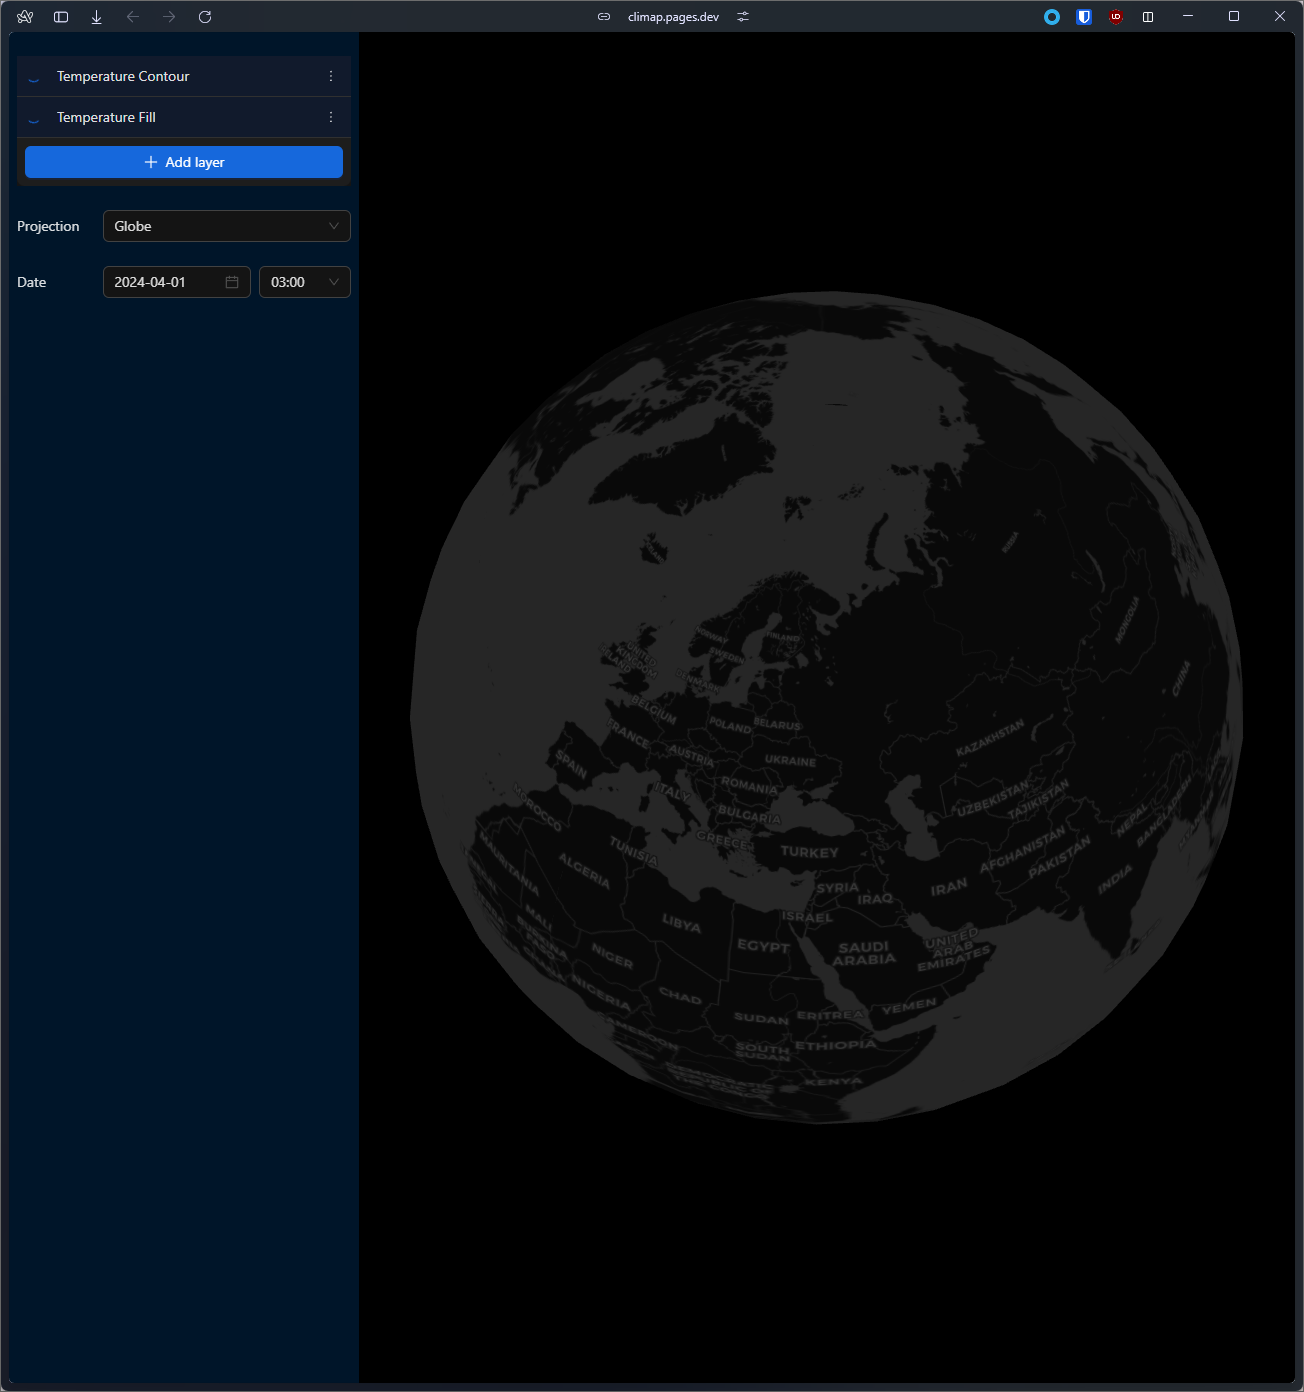
\includegraphics[width=15cm]{./assets/pic1.png}
		\caption{Главное окно программы}
	\end{figure}

	\subsection{Добавление слоев}
	Для добавления слоя необходимо нажать на кнопку <<Добавить слой>> или <<Add layer>> в панели настроек в левой части
	приложения. По-умолчанию при первой загрузке выбраны стандартные слои с данными по средней температуре -- сплошная
	заливка и контур (изолинии).

	После нажатия на кнопку появится меню выбора данных и параметров слоя:
	\begin{figure}[!h]
		\centering
		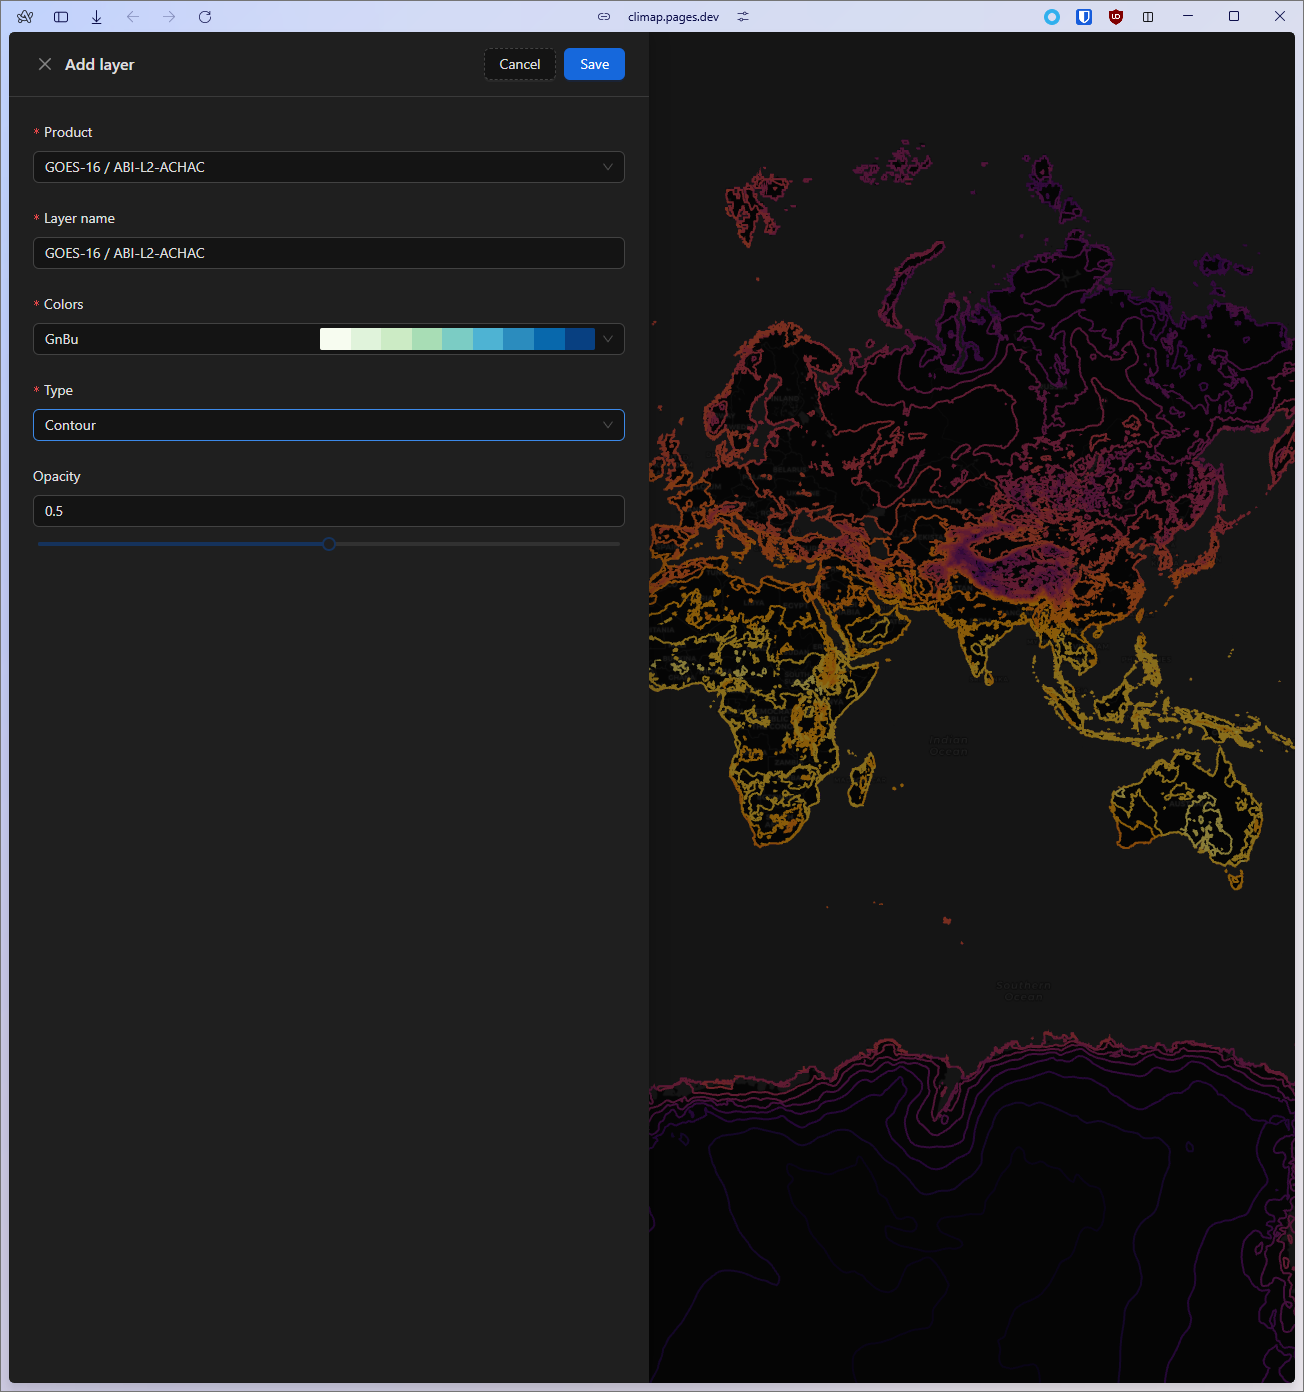
\includegraphics[width=15cm]{./assets/pic2.png}
		\caption{Окно настроек слоя}
	\end{figure}

	Оператору необходимо выбрать набор данных из выпадающего вложенного списка, также возможно фильтровать даныные по подстроке,
	вводя текст при активированном списке выбора данных.

	\begin{figure}[h!]
		\centering
		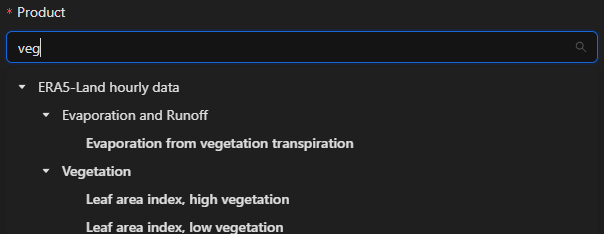
\includegraphics[width=8cm]{./assets/pic3.png}
		\caption{Поиск и выбор данных}
	\end{figure}

	Другие поля предназначены для выбора названия слоя (текст, по умолчанию - название источника данных), палитра заливки или
	контура, тип отображения, прозрачность слоя (где 1 - полностью непрозрачный, 0 - полностью прозрачный).

	После настройки всех параметров, для добавления слоя необходимо нажать кнопку <<Сохранить>> (<<Save>>), после чего
	создастся новый слой в списке текущих слоев. При нажатии на кнопку <<Отмена>> (<<Cancel>>) слой не будет сохранен.
	После этого окно настроек слоя закроется.

	Слева от названия каждого слоя присутствуют соответствующие индикаторы. Сразу после добавления слоя будет отображаться
	индикатор загрузки -- вращающийся круг, до тех пор, пока данные не загрузятся и слой не будет отрисован. При ошибке загрузки
	будет отображен желтый индикатор <<Внимание>>, по наведении на который будет отображена ошибка в виде всплывающего
	текста. После успешной загрузки слоя рядом с ним будет присутствовать флажок -- галочка на синем фоне (слой отображается)
	или прозрачный квадрат (слой скрыт), по нажатии на которые можно переключать видимость слоя.

	\begin{figure}[h!]
		\centering
		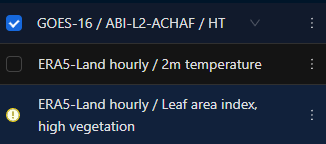
\includegraphics{./assets/pic5.png}
		\caption{Индикаторы статуса слоя}
	\end{figure}

	Некоторые наборы данных содержат несколько переменных, которые будут обнаружены только после загрузки, например
	датасеты GOES-16 содержат дополнительную переменную <<DQF>>, в которой записаны показатели качества данных в различных
	областях. Такие переменные также можно использовать для отображения, выбрав их в выпадающем списке, появляющемся по
	нажатии на слой.

	\begin{figure}[h!]
		\centering
		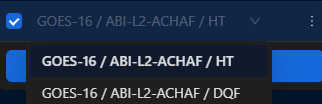
\includegraphics{./assets/pic4.png}
		\caption{Выбор переменной}
	\end{figure}

	\subsection{Редактирования слоев}
	Существующие слои можно редактировать, нажав на <<\vdots>> справа от названия. При этом откроется то же окно, что и
	при создании слоя, но с дополнительной кнопкой <<Удалить слой>> (<<Remove layer>>), по нажатии на которую слой будет
	удален из списка и перестанет отображаться.

	\subsection{Глобальные параметры}
	Все данные отображаются на карте с одинаковым набором глобальных параметров, таких как:
	\begin{itemize}
		\item проекция -- трехмерный глобус или плоская проекция меркатора;

		\item дата и время с точностью до одного часа (для данных с частотой обновления менее одного часа будет отображаться
			ближайшее доступное время).
	\end{itemize}
	Параметры можно выбирать с помощью соответствующих полей:
	\begin{figure}[h!]
		\centering
		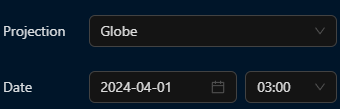
\includegraphics{./assets/pic6.png}
		\caption{Выбор глобальных параметров}
	\end{figure}
\end{document}